%%%%%%%%%%%%%%%%%%%%%%%%%%%%%%%%%%%%%%%%%
% Classicthesis Typographic Thesis
% LaTeX Template
% Version 1.3 (15/2/14)
%
% André Miede (http://www.miede.de)
%
%%%%%%%%%%%%%%%%%%%%%%%%%%%%%%%%%%%%%%%%%

\documentclass[
		twoside,openright,titlepage,numbers=noenddot,headinclude,%1headlines,
                footinclude=true,cleardoublepage=empty,
                BCOR=5mm,paper=a4,fontsize=11pt, % Binding correction, paper type and font size
                ngerman,american, % Languages
                ]{scrreprt} 
\usepackage[utf8]{inputenc}
\usepackage{shadethm}


%Stuff for definitions using shadethm
\newshadetheorem{definitions}{Definition}[chapter]
\newenvironment{definition}[1][]{%
  \definecolor{shadethmcolor}{rgb}{.9,.9,.95}%
  \definecolor{shaderulecolor}{rgb}{0.0,0.0,0.4}%
%  \setlength{\shadeboxrule}{1.5pt}%
  \begin{definitions}[#1]\hspace*{2mm}%
}{\end{definitions}}

%%%%%%%%%%%%%%%%%%%%%%%%%%%%%%%%%%%%%%%%%
% Thesis Configuration File
%
% The main lines to change in this file are in the DOCUMENT VARIABLES
% section, the rest of the file is for advanced configuration.
%
%%%%%%%%%%%%%%%%%%%%%%%%%%%%%%%%%%%%%%%%%

%----------------------------------------------------------------------------------------
%	DOCUMENT VARIABLES
%	Fill in the lines below to enter your information into the thesis template
%	Each of the commands can be cited anywhere in the thesis
%----------------------------------------------------------------------------------------

% Remove drafting to get rid of the '[ Date - classicthesis version 4.0 ]' text at the bottom of every page
\PassOptionsToPackage{eulerchapternumbers,listings,drafting, pdfspacing, subfig,beramono,eulermath,parts}{classicthesis}
% Available options: drafting parts nochapters linedheaders eulerchapternumbers beramono eulermath pdfspacing minionprospacing tocaligned dottedtoc manychapters listings floatperchapter subfig
% Adding 'dottedtoc' will make page numbers in the table of contents flushed right with dots leading to them

\newcommand{\myTitle}{Multi-episodic Subjective Quality with Telecommunication Services\xspace}
\newcommand{\mySubtitle}{An Homage to The Elements of Typographic Style\xspace}
\newcommand{\myDegree}{Doktor-Ingenieur (Dr.-Ing.)\xspace}
\newcommand{\myName}{Dennis Guse\xspace}
\newcommand{\myProf}{Prof. Dr.-Ing. Sebastian Möller\xspace}
\newcommand{\myOtherProf}{tbd\xspace}
\newcommand{\mySupervisor}{\xspace}
\newcommand{\myFaculty}{Fakultät IV\xspace}
\newcommand{\myDepartment}{Quality and Usability Lab\xspace}
\newcommand{\myUni}{Technische Universität Berlin\xspace}
\newcommand{\myLocation}{Berlin\xspace}
\newcommand{\myTime}{April 2016\xspace}
\newcommand{\myVersion}{version 4.0\xspace}

%----------------------------------------------------------------------------------------
%	USEFUL COMMANDS
%----------------------------------------------------------------------------------------

\newcommand{\ie}{i.\,e.}
\newcommand{\Ie}{I.\,e.}
\newcommand{\eg}{e.\,g.}
\newcommand{\Eg}{E.\,g.} 

\newcounter{dummy} % Necessary for correct hyperlinks (to index, bib, etc.)
\providecommand{\mLyX}{L\kern-.1667em\lower.25em\hbox{Y}\kern-.125emX\@}

%----------------------------------------------------------------------------------------
%	PACKAGES
%----------------------------------------------------------------------------------------

\usepackage{lipsum} % Used for inserting dummy 'Lorem ipsum' text into the template

%------------------------------------------------
 
\PassOptionsToPackage{latin9}{inputenc} % latin9 (ISO-8859-9) = latin1+"Euro sign"
\usepackage{inputenc}
 
 %------------------------------------------------

%\PassOptionsToPackage{ngerman,american}{babel}  % Change this to your language(s)
% Spanish languages need extra options in order to work with this template
%\PassOptionsToPackage{spanish,es-lcroman}{babel}
\usepackage{babel}

%------------------------------------------------			

\PassOptionsToPackage{square,numbers}{natbib}
 \usepackage{natbib}
 
 %------------------------------------------------

\PassOptionsToPackage{fleqn}{amsmath} % Math environments and more by the AMS 
 \usepackage{amsmath}
 
 %------------------------------------------------

\PassOptionsToPackage{T1}{fontenc} % T2A for cyrillics
\usepackage{fontenc}

%------------------------------------------------

\usepackage{xspace} % To get the spacing after macros right

%------------------------------------------------

\usepackage{mparhack} % To get marginpar right

%------------------------------------------------

\usepackage{fixltx2e} % Fixes some LaTeX stuff 

%------------------------------------------------

\PassOptionsToPackage{smaller}{acronym} % Include printonlyused in the first bracket to only show acronyms used in the text
\usepackage{acronym} % nice macros for handling all acronyms in the thesis

%------------------------------------------------

%\renewcommand*{\acsfont}[1]{\textssc{#1}} % For MinionPro
%\renewcommand{\bflabel}[1]{{#1}\hfill} % Fix the list of acronyms

%------------------------------------------------

\PassOptionsToPackage{pdftex}{graphicx}
\usepackage{graphicx} 

%----------------------------------------------------------------------------------------
%	FLOATS: TABLES, FIGURES AND CAPTIONS SETUP
%----------------------------------------------------------------------------------------

\usepackage{tabularx} % Better tables
\setlength{\extrarowheight}{3pt} % Increase table row height
\newcommand{\tableheadline}[1]{\multicolumn{1}{c}{\spacedlowsmallcaps{#1}}}
\newcommand{\myfloatalign}{\centering} % To be used with each float for alignment
\usepackage{caption}
\captionsetup{format=hang,font=small}
\usepackage{subfig}  

%----------------------------------------------------------------------------------------
%	CODE LISTINGS SETUP
%----------------------------------------------------------------------------------------

\usepackage{listings} 
%\lstset{emph={trueIndex,root},emphstyle=\color{BlueViolet}}%\underbar} % for special keywords
\lstset{language=[LaTeX]Tex, % Specify the language for listings here
keywordstyle=\color{RoyalBlue}, % Add \bfseries for bold
basicstyle=\small\ttfamily, % Makes listings a smaller font size and a different font
%identifierstyle=\color{NavyBlue}, % Color of text inside brackets
commentstyle=\color{Green}\ttfamily, % Color of comments
stringstyle=\rmfamily, % Font type to use for strings
numbers=left, % Change left to none to remove line numbers
numberstyle=\scriptsize, % Font size of the line numbers
stepnumber=5, % Increment of line numbers
numbersep=8pt, % Distance of line numbers from code listing
showstringspaces=false, % Sets whether spaces in strings should appear underlined
breaklines=true, % Force the code to stay in the confines of the listing box
%frameround=ftff, % Uncomment for rounded frame
frame=single, % Frame border - none/leftline/topline/bottomline/lines/single/shadowbox/L
belowcaptionskip=.75\baselineskip % Space after the "Listing #: Desciption" text and the listing box
}

%----------------------------------------------------------------------------------------
%	HYPERREFERENCES
%----------------------------------------------------------------------------------------

\PassOptionsToPackage{pdftex,hyperfootnotes=false,pdfpagelabels}{hyperref}
\usepackage{hyperref}  % backref linktocpage pagebackref
\pdfcompresslevel=9
\pdfadjustspacing=1

\hypersetup{
% Uncomment the line below to remove all links (to references, figures, tables, etc)
%draft, 
colorlinks=true, linktocpage=true, pdfstartpage=3, pdfstartview=FitV,
% Uncomment the line below if you want to have black links (e.g. for printing black and white)
%colorlinks=false, linktocpage=false, pdfborder={0 0 0}, pdfstartpage=3, pdfstartview=FitV, 
breaklinks=true, pdfpagemode=UseNone, pageanchor=true, pdfpagemode=UseOutlines,
plainpages=false, bookmarksnumbered, bookmarksopen=true, bookmarksopenlevel=1,
hypertexnames=true, pdfhighlight=/O, urlcolor=webbrown, linkcolor=RoyalBlue, citecolor=webgreen,
%------------------------------------------------
% PDF file meta-information
pdftitle={\myTitle},
pdfauthor={\textcopyright\ \myName, \myUni, \myFaculty},
pdfsubject={},
pdfkeywords={},
pdfcreator={pdfLaTeX},
pdfproducer={LaTeX with hyperref and classicthesis}
%------------------------------------------------
}   

%----------------------------------------------------------------------------------------
%	BACKREFERENCES
%----------------------------------------------------------------------------------------

\usepackage{ifthen} % Allows the user of the \ifthenelse command
\newboolean{enable-backrefs} % Variable to enable backrefs in the bibliography
\setboolean{enable-backrefs}{false} % Variable value: true or false

\newcommand{\backrefnotcitedstring}{\relax} % (Not cited.)
\newcommand{\backrefcitedsinglestring}[1]{(Cited on page~#1.)}
\newcommand{\backrefcitedmultistring}[1]{(Cited on pages~#1.)}
\ifthenelse{\boolean{enable-backrefs}} % If backrefs were enabled
{
\PassOptionsToPackage{hyperpageref}{backref}
\usepackage{backref} % to be loaded after hyperref package 
\renewcommand{\backreftwosep}{ and~} % separate 2 pages
\renewcommand{\backreflastsep}{, and~} % separate last of longer list
\renewcommand*{\backref}[1]{}  % disable standard
\renewcommand*{\backrefalt}[4]{% detailed backref
\ifcase #1 
\backrefnotcitedstring
\or
\backrefcitedsinglestring{#2}
\else
\backrefcitedmultistring{#2}
\fi}
}{\relax} 

%----------------------------------------------------------------------------------------
%	AUTOREFERENCES SETUP
%	Redefines how references in text are prefaced for different 
%	languages (e.g. "Section 1.2" or "section 1.2")
%----------------------------------------------------------------------------------------

\makeatletter
\@ifpackageloaded{babel}
{
\addto\extrasamerican{
\renewcommand*{\figureautorefname}{Figure}
\renewcommand*{\tableautorefname}{Table}
\renewcommand*{\partautorefname}{Part}
\renewcommand*{\chapterautorefname}{Chapter}
\renewcommand*{\sectionautorefname}{Section}
\renewcommand*{\subsectionautorefname}{Section}
\renewcommand*{\subsubsectionautorefname}{Section}
}
\addto\extrasngerman{
\renewcommand*{\paragraphautorefname}{Absatz}
\renewcommand*{\subparagraphautorefname}{Unterabsatz}
\renewcommand*{\footnoteautorefname}{Fu\"snote}
\renewcommand*{\FancyVerbLineautorefname}{Zeile}
\renewcommand*{\theoremautorefname}{Theorem}
\renewcommand*{\appendixautorefname}{Anhang}
\renewcommand*{\equationautorefname}{Gleichung}
\renewcommand*{\itemautorefname}{Punkt}
}
\providecommand{\subfigureautorefname}{\figureautorefname} % Fix to getting autorefs for subfigures right
}{\relax}
\makeatother

%----------------------------------------------------------------------------------------

\usepackage{classicthesis} 

%----------------------------------------------------------------------------------------
%	CHANGING TEXT AREA 
%----------------------------------------------------------------------------------------

%\linespread{1.05} % a bit more for Palatino
%\areaset[current]{312pt}{761pt} % 686 (factor 2.2) + 33 head + 42 head \the\footskip
%\setlength{\marginparwidth}{7em}%
%\setlength{\marginparsep}{2em}%

%----------------------------------------------------------------------------------------
%	USING DIFFERENT FONTS
%----------------------------------------------------------------------------------------

%\usepackage[oldstylenums]{kpfonts} % oldstyle notextcomp
%\usepackage[osf]{libertine}
%\usepackage{hfoldsty} % Computer Modern with osf
%\usepackage[light,condensed,math]{iwona}
%\renewcommand{\sfdefault}{iwona}
%\usepackage{lmodern} % <-- no osf support :-(
%\usepackage[urw-garamond]{mathdesign} <-- no osf support :-(

\begin{document}

\frenchspacing % Reduces space after periods to make text more compact
\raggedbottom % Makes all pages the height of the text on that page
\selectlanguage{american} % Select your default language - e.g. american or ngerman

%\renewcommand*{\bibname}{new name} % Uncomment to change the name of the bibliography
%\setbibpreamble{} % Uncomment to include a preamble to the bibliography - some text before the reference list starts

\pagenumbering{roman} % Roman page numbering prior to the start of the thesis content (i, ii, iii, etc)
\pagestyle{plain} % Suppress headers for the pre-content pages

%----------------------------------------------------------------------------------------
%	PRE-CONTENT THESIS PAGES
%----------------------------------------------------------------------------------------

\renewcommand*{\cleardoublepage}{}

% Title Page

\begin{titlepage}

\begin{addmargin}[-1cm]{-3cm}
\begin{center}
\large

\hfill
\vfill

\begingroup
\color{Maroon}\spacedallcaps{\myTitle} \\ \bigskip % Thesis title
\endgroup

\spacedlowsmallcaps{\myName} % Your name

\vfill

\mySubtitle \\ \medskip % Thesis subtitle
%\myDegree \\
%\myDepartment \\
%\myFaculty \\
%\myUni \\ \bigskip

%\myTime\ -- \myVersion % Time and version

\vfill

\end{center}
\end{addmargin}

\end{titlepage} % Main title page
%% Back of the title page

\thispagestyle{empty}

\hfill

\vfill

\noindent\myName: \textit{\myTitle,} \mySubtitle, %\myDegree, 
\textcopyright\ \myTime

% You may wish to do something with the back of the title page, such as including your supervisors, location or time frame of the work. Below is an example of doing so although you may want to tweak it to your liking.

%\bigskip

%\noindent\spacedlowsmallcaps{Supervisors}: \\
%\myProf \\
%\myOtherProf \\ 
%\mySupervisor

%\medskip \\

%\noindent\spacedlowsmallcaps{Location}: \\
%\myLocation

%\medskip \\

%\noindent\spacedlowsmallcaps{Time Frame}: \\
%\myTime
 % Back of the title page
%\cleardoublepage% Dedication

\thispagestyle{empty}
\refstepcounter{dummy}

\pdfbookmark[1]{Dedication}{Dedication} % Bookmark name visible in a PDF viewer

\vspace*{3cm}

\begin{center}
The remembering self is sometimes simply wrong. \\ \medskip
--- (Kahneman and Riss, 2005, p. 286)
\end{center}

\medskip

\begin{center}
Experiences are fleeting [whereas] memories are what we get to from our experiences. \\ \medskip

--- Mrion-Shatz et al. 2009 after Kahneman & Riis 2005, p. 286 (Not present here!)
\end{center}
 % Dedication page
%\cleardoublepage\include{support/FrontBackMatter/Foreword} % Uncomment and create a Foreword.tex to include a foreword
%\cleardoublepage% Abstract

\pdfbookmark[1]{Abstract}{Abstract} % Bookmark name visible in a PDF viewer

\begingroup
\let\clearpage\relax
\let\cleardoublepage\relax
\let\cleardoublepage\relax

\chapter*{Abstract} % Abstract name

Short summary of the contents\dots

\endgroup			

\vfill % Abstract page
%\cleardoublepage% Publications - a page listing research articles written using content in the thesis

\pdfbookmark[1]{Publications}{Publications} % Bookmark name visible in a PDF viewer

\chapter*{Publications} % Publications page text

Some ideas and figures have appeared previously in the following publications:

\bigskip

\noindent Put your publications from the thesis here. The packages \texttt{multibib} or \texttt{bibtopic} etc. can be used to handle multiple different bibliographies in your document. % Publications from the thesis page
%\cleardoublepage% Acknowledgements

\pdfbookmark[1]{Acknowledgements}{Acknowledgements} % Bookmark name visible in a PDF viewer

\begin{flushright}{\slshape    
We have seen that computer programming is an art, \\ 
because it applies accumulated knowledge to the world, \\ 
because it requires skill and ingenuity, and especially \\
because it produces objects of beauty.} \\ \medskip
--- \defcitealias{knuth:1974}{Donald E. Knuth}\citetalias{knuth:1974} \citep{knuth:1974}
\end{flushright}

\bigskip

%----------------------------------------------------------------------------------------

\begingroup

\let\clearpage\relax
\let\cleardoublepage\relax
\let\cleardoublepage\relax

\chapter*{Acknowledgements} % Acknowledgements section text

Put your acknowledgements here.\\

\noindent Many thanks to everybody who already sent me a postcard!\\

\noindent Regarding the typography and other help, many thanks go to Marco Kuhlmann, Philipp Lehman, Lothar Schlesier, Jim Young, Lorenzo Pantieri and Enrico Gregorio\footnote{Members of GuIT (Gruppo Italiano Utilizzatori di \TeX\ e \LaTeX )}, J\"org Sommer, Joachim K\"ostler, Daniel Gottschlag, Denis Aydin, Paride Legovini, Steffen Prochnow, Nicolas Repp, Hinrich Harms, Roland Winkler,  and the whole \LaTeX-community for support, ideas and some great software.

\bigskip

\noindent\emph{Regarding \mLyX}: The \mLyX\ port was intially done by
\emph{Nicholas Mariette} in March 2009 and continued by
\emph{Ivo Pletikosi\'c} in 2011. Thank you very much for your work and the contributions to the original style.

\endgroup % Acknowledgements page
%\pagestyle{scrheadings} % Show chapter titles as headings
%\cleardoublepage% Table of Contents - List of Tables/Figures/Listings and Acronyms

\refstepcounter{dummy}

\pdfbookmark[1]{\contentsname}{tableofcontents} % Bookmark name visible in a PDF viewer

\setcounter{tocdepth}{2} % Depth of sections to include in the table of contents - currently up to subsections

\setcounter{secnumdepth}{3} % Depth of sections to number in the text itself - currently up to subsubsections

\manualmark
\markboth{\spacedlowsmallcaps{\contentsname}}{\spacedlowsmallcaps{\contentsname}}
\tableofcontents 
\automark[section]{chapter}
\renewcommand{\chaptermark}[1]{\markboth{\spacedlowsmallcaps{#1}}{\spacedlowsmallcaps{#1}}}
\renewcommand{\sectionmark}[1]{\markright{\thesection\enspace\spacedlowsmallcaps{#1}}}

\clearpage

\begingroup 
\let\clearpage\relax
\let\cleardoublepage\relax
\let\cleardoublepage\relax

%----------------------------------------------------------------------------------------
%	List of Figures
%----------------------------------------------------------------------------------------

\refstepcounter{dummy}
%\addcontentsline{toc}{chapter}{\listfigurename} % Uncomment if you would like the list of figures to appear in the table of contents
\pdfbookmark[1]{\listfigurename}{lof} % Bookmark name visible in a PDF viewer

%TODO \listoffigures

\vspace*{8ex}
\newpage

%----------------------------------------------------------------------------------------
%	List of Tables
%----------------------------------------------------------------------------------------

\refstepcounter{dummy}
%\addcontentsline{toc}{chapter}{\listtablename} % Uncomment if you would like the list of tables to appear in the table of contents
\pdfbookmark[1]{\listtablename}{lot} % Bookmark name visible in a PDF viewer

%TODO \listoftables
        
\vspace*{8ex}
\newpage
    
%----------------------------------------------------------------------------------------
%	List of Listings
%---------------------------------------------------------------------------------------- 

\refstepcounter{dummy}
%\addcontentsline{toc}{chapter}{\lstlistlistingname} % Uncomment if you would like the list of listings to appear in the table of contents
\pdfbookmark[1]{\lstlistlistingname}{lol} % Bookmark name visible in a PDF viewer

%TODO \lstlistoflistings 

\vspace*{8ex}
\newpage
       
%----------------------------------------------------------------------------------------
%	Acronyms
%----------------------------------------------------------------------------------------

\refstepcounter{dummy}
%\addcontentsline{toc}{chapter}{Acronyms} % Uncomment if you would like the acronyms to appear in the table of contents
\pdfbookmark[1]{Acronyms}{acronyms} % Bookmark name visible in a PDF viewer

\markboth{\spacedlowsmallcaps{Acronyms}}{\spacedlowsmallcaps{Acronyms}}

\chapter*{Acronyms}
\begin{acronym}[MUSHRA]
\acro{QoE}{Quality of Experience}
\acro{MOS}{Mean Opinion Score}
\acro{MUSHRA}{Multi-Stimulus Test with Hidden Reference and Anchor}
\acro{ACR}{Absolute Category Rating}
\acro{DCR}{Degradation Category Rating}
\acro{LOT}{Listening-only test}
\acro{CT}{Conversation test}
\acro{NPS}{Net Promoter Score}
\acro{EEG}{Electroencephalography}
\acro{SCT}{Short Conversation Test}

\acro{API}{Application Programming Interface}
\acro{IP}{Internet Protocol}
\acro{QoS}{Quality of Service}
\acro{HTML}{Hypertext Markup Language}
\acro{HTTP}{Hypertext Transfer Protocol}
\acro{RTP}{Real-Time Transport Protocol}
\acro{VoIP}{Voice-over-IP}
\acro{SIP}{Session Initiation Protocol}
\acro{STUN}{Session Traversal Utilities for NAT}

\acro{SIM}{Subscriber Identity Module}
\acro{GSM}{Global System for Mobile Communications}
\acro{MP3}{MPEG-1 Audio Layer III}
\acro{H.264}{MPEG-4 Part 10, Advanced Video Coding}

\acro{ITU}{Internation Telecommunications Union}
\acro{ETSI}{European Telecommunications Standards Institute}
\end{acronym}  
                   
\endgroup % Contents, list of figures/tables/listings and acronyms

\cleardoublepage

%----------------------------------------------------------------------------------------
%	THESIS CONTENT - CHAPTERS
%----------------------------------------------------------------------------------------

\part{Introduction and State of the Art}\cleardoublepage
\pagenumbering{arabic} % Arabic page numbering for thesis content (1, 2, 3, etc)
\setcounter{page}{1} % Uncomment to manually start the page counter at an arbitrary value (for example if you wish to count the pre-content pages in the page count)
\chapter{Introduction}\label{chap:01}

\section{Motivation}
In contrast to products, which can be manufactured and stored, a service is created on demand.
A service is simultaneously produced by the \emph{service provider} and consumed by the \emph{customer}.
A typical example is a \emph{telecommunication service} like speech telephony, or Internet access.
%US Communications Act 1934
Telecommunication services provide communication between one or more parties in form of data transmission.
Here, a party can be a person, but also a computer.
A service provider maintains the network infrastructure to provide telecommunication services and makes it available to potential users\footnote{Throughout this thesis persons engaged in a service are called \emph{users} of this service without distinction if they are the actual customers.}.
An actual service is produced when a user interacts with a telecommunication service.

As a service is produced when it is used, the provided \emph{performance} might be varying within a usage instance as well as between distinct usage instances.
Here, performance are absolutely measurable parameters of this service like transmission bandwidth and one-way transmission delay~\citep[][p. 12]{moller_assessment_2000}.
In case of a telecommunication service, varying performance can be the result of current network load conditions, network equipment failure, but also related to end-user devices.
The usage of telecommunication services can be divided into two aspects.
First, a user can actively interact with a service like starting and engaging a telephone conversation.
Second, a service can also be used passively, \eg, providing reachability of a telephone.

The active use of a telecommunication service results in a \emph{perceived quality} of this interaction.
It is assumed that perceived quality results from a comparison between the \emph{desired experience} and \emph{actual experience} \citep[][p.~13]{raake_quality_2014}. %Expected experience?
Experience includes all perceptions resulting from this service instance \citep[][p.~13]{raake_quality_2014}.
The perceived quality of an interaction with a service is affected by the experienced performance, but also by individual factors like expectations, usage situation, etc \citep[\eg,][p.~55ff.]{reiter_factors_2014}.

%QoE Methods; human perception 
Understanding the relationship between performance of a service and perceived quality has become an important field of research investigating the so-called \ac{QoE}.
Starting from speech transmission for telephony \citep[][]{ieee_audio_and_electroacoustics_group_ieee_1969} and its inherent impairments, \ac{QoE} now mainly considers digital transmission of multimedia data. % \citep{moller_quality_2014}.
This includes the production, coding, transmission, decoding and reproduction of text, voice, speech, audio, image and video information.
Specific characteristics of human perceptual systems have been used to develop enhanced coding mechanisms like \ac{MP3} and \ac{H.264}.
These apply compression to provide a reduction in data rate while maintain only little reduction in perceived quality.

Another application of knowledge about \ac{QoE} is the monitoring of network transmission infrastructure.
This allows to estimate the actual impact of provided performance on a user.
Such knowledge enables a service provider to react accordingly to avoid reductions in perceived quality.
For example, in case of a video streaming service stalling, provoked by a temporary reduction in network bandwidth, could be avoided by reducing the transmission bandwidth.
Although perceived quality is likely to be affected, the service is still provided and remains useful for the user.

%Service choice
In general, a user can choose from a variety of service providers, which provide a similar service, and select the one provider that suits his needs best.
For a reasonable selection a user must know his needs, requirements, economical limits and estimate the perceived quality (\ie, \emph{assumed quality}) \citep[][p.~13]{raake_quality_2014}.
Based upon this knowledge he can estimate, if the usage of a service is likely to be satisfying for him.
After experiencing an interaction with a service, the user can then evaluate, if this service fulfills his needs including his perceived quality.
He can then decide to use the service again or rather select a different service provider, when he needs this type of service again~\citep[][]{geerts_linking_2010}.

\section{Research Question}
Of special interest is the perception of varying performance over distinct interactions with one service and the resulting perceived quality.
%This is, in fact, a common case for telecommunication service(s).
%For example a user of a mobile telephony provider will use the provided service(s) usually repeatedly as his telephone number is bound to the service provider.
Especially for telecommunication services the impact of varying performance from usage instance to usage instance is of interest.
Although the impact of varying performance during one usage episode has been investigated, it is so far not known how perceived quality evolves over several distinct episodes (\ie, individual experiences).
This is one factor that contributes to the \emph{service quality} of a service \citep[][]{berry_quality_1985, zeithaml_behavioral_1996}.
The construct of service quality maintains a holistic view from a business perspective of service usage focusing on aspects like customer loyalty \citep{parasuraman_conceptual_1985}.
%In fact, perceived quality is an implicit part of service quality.

This thesis investigates perceived quality over several distinct and meaningful interactions with a service.
Such an interaction is denoted as \emph{usage episode} (\cf, \autoref{chap:03}).
The quality of a usage episode is denoted as \emph{episodic quality}.
The perceived quality over several distinct usage episodes is denoted as \emph{multi-episodic perceived quality}.

This particular thesis addresses the following research question: 
\subparagraph*{Research Question:}
How does multi-episodic quality for one user evolves over several usage episodes with one service?

\subparagraph*{}
%Memory
%Each usage episode results in a perceived quality, which can be assessed momentary during the usage episode and also in retrospective after the usage episode is finished.
So far, the integration process of perceived quality of distinct usage episodes into a multi-episodic perceived quality is not yet known.
It could be a continuous process that integrates current experiences immediately into a current view, or a retrospective assessment evaluating all memorized and recallable information \citep[][]{hogarth_order_1992}. 
In fact, it could also be a mixture of both.

%%%I focus on telecommunication services(s) as those are well-studied with regard to perceived quality, are widely used, and variations in performance, irrespective of the actual reason, occur relative frequently.

\section{Goals}
In this thesis, I pursue two goals towards understanding the formation process of multi-episodic perceived quality.
I will focus solely on telecommunication services, because those are prone to variations in performance and usage episodes are relatively short.
As the formation process of multi-episodic perceived quality cannot be observed directly (\cf, \autoref{chap:02}), this investigation will rely on the judgments of multi-episodic perceived quality.
%This investigation will rely on judgments of multi-episodic perceived quality alone as perceived quality cannot be observed directly (\cf, \autoref{chap:02}).

This leads to two goals:

\subparagraph*{Goal 1:}
%I will investigate how episodic performance determines the judgment of multi-episodic perceived quality and investigate potential anomalies of the formation process.
I will investigate how the performance of a sequence of usage episodes determines judgments of multi-episodic perceived quality.

\subparagraph*{Goal 2:}
I will investigate how multi-episodic judgments can be predicted based upon episodic judgments.

\subparagraph*{}
I will conduct this investigation for different \emph{usage periods}.
Usage periods denotes the time frame in which a user interacts repeatedly with a service.
Here, I consider two usage periods.
First, I investigate multi-episodic perceived quality in one session consisting of several usage episodes.
Second, I investigated multi-episodic perceived quality several days.
This is necessary, because it is not known if the time between usage episodes affects the formation process of multi-episodic perceived quality.

\section{Structure}
This thesis is structured as follows.
In \autoref{chap:02}, I introduce concepts and fundamentals that form the basis for my investigation of multi-episodic perceived quality.
It starts with an introduction to psychophysics and \ac{QoE}, followed by an introduction into human memory and known biases for retrospective judgments.
Then, the state of the art on perceived quality and performance fluctuations is presented.
Finally, the prior work on multi-episodic perceived quality is presented and discussed.
%Here, the assessment method developed by \citet{moller_single-call_2011}, which is the following denoted as \emph{defined-use}, is presented in detail.

Then, I present my work towards multi-episodic perceived quality. % based upon the defined use method.
In \autoref{chap:towards}, I describe the selected aspects of the defined-use method and the to be investigated hypotheses.
Those hypotheses are the basis for my investigations on multi-episodic perceived quality in one session (\autoref{chap:lab}) as well as over several days (\autoref{chap:field}).
%Those different time frames are necessary to investigate as it is not known, if the time between usage episodes affect the formation process.
Based upon the conducted experiments, I investigate potential models for the prediction of multi-episodic judgments based upon prior episodic judgments (\autoref{chap:modeling}).
Finally, I summarize my thesis, discuss the results and present directions for future work in \autoref{chap:discussion}.
\section{Perceptual Quality}
\subsection{Perception and Psychophysics}
Humans use their senses, \ie, perceptual organs, to perceive events of their environment.
Based upon those events, an internal model is created and updated, which incorporates knowledge about the environment.
%This model is used to plan actions and updated when new information, including perceptual events, are processed~\citep[p.~4]{blauert_spatial_1996}.
A \emph{perceptual event} occurs in a human observer, when a \emph{physical event} stimulates a sensory organ~\citep[p.~5]{blauert_spatial_1996}.
A physical event is an observable occurrence in time, location and character~\citep{le_callet_qualinet_2013}.
%One example of a physical event is a sound event that reaches the ear results in an auditory event in the observer (see \autoref{img:chap02:auditory-event}).
A perceptual event cannot be observed directly, because it occurs inside the observer due to perceptual and mental processing.
It can, however, be described by the observer.
The description process requires that a perceptual event can be observed consciously.
In addition, a perceptual event can also be observed indirectly with behavioral measurements and physiological measurements.
In fact, these measurements might be considered a special form of description.
A psychometric function can be derived by measuring the properties of physical events and relating those to the description.

A psychophysical experiment is conducted by presenting one or more physical events as stimuli to one or more observers.
Each individual observer derives the description of his perceptual event.
A description can be expressed in a quantitative form, by selecting the best fitting answer from a predefined set, or in a free form.
For different observers the description the perceptual event resulting from a physical event must not necessarily be identical.
In fact, each observer describes his individual perceptual event with regard to his concepts~\citep[p.~11]{blauert_spatial_1996}.
%A psychophysical experiment is considered \emph{objective}, if the results are reproducible independent if one observer is measured or multiple observers~\citep[p. 11]{blauert_spatial_1996}.

The perception of a physical event may change the internal state of an observer \citep{raake_quality_2014}.
A physical event reaching the sensory organ can affect the sensitivity of this organ, or the observer might react to a physical event.
Thus, the perception of following physical events might be affected.
Also, the description of successive stimuli might be affected by presentation order, because previous stimuli can be used as reference.
%The perception of different physical events is not only affected by the temporal order, but temporal close physical events may be grouped together and form one perceptual event.
Beside this, also the \emph{active} observation might affect the perceptual process \citep[][p.~30]{raake_quality_2014}.
Here, an observer might focus his attention on the perception to derive a description of a perceptual event.
This might actually influence resulting perceptual events and thus the description.


\subsection{Perceptual Quality and Formation Process}\label{related:perceivedQuality}
Perceptual quality is a branch of psychophysics focusing on the experience due to perception and the resulting quality of this experience.
\begin{definition}[Experiencing]
``is the individual stream of perceptions (of feelings, sensory percepts and concepts) that occurs in a particular situation of reference.''~\citep[p.~13]{raake_quality_2014}.
\end{definition}

With regard to the quality of an experience and the underlying perceptual events, \citet{jekosch_voice_2005} formulates the \emph{quality formation process} as an individual comparison process between the desired, or expected, outcome with the experienced outcome.
The comparison of expectations and the actual experience results in a \emph{quality event} in the observer.
%This complements the description of a perceptual event by an additional quality evaluation process.
%This process is shown in \autoref{img:chap02:quality-event}.
%\begin{figure}
%	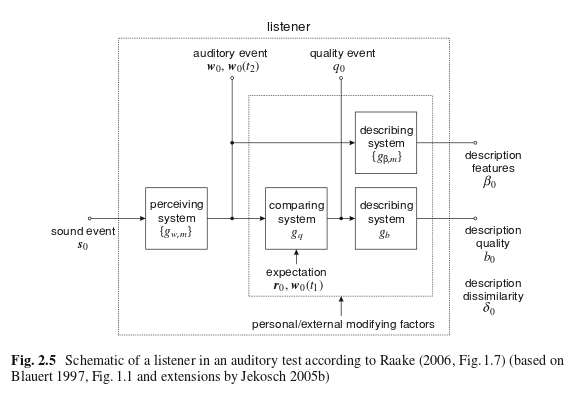
\includegraphics[width=1\textwidth]{figure/quality-event}
%	\caption{Quality formation and description process as extension to the perceptual event taken from \citet{waltermann_dimension-based_2013} after \citet{raake_short-_2006}.}
%	\label{img:chap02:quality-event} %Waeltermann, 2013
%\end{figure}
It is assumed that a perceptual event is evaluated by a \emph{comparing system} within an observer.
This system  derives the \emph{quality features} of this event~\citep[\cf,][p.~17]{jekosch_voice_2005}.\footnote{\citet{jekosch_voice_2005} uses the term \emph{entity} with regard to the quality formation process.
As entity does not convey a temporal component, the term \emph{event} is in this work used instead; following the notion of \citet{blauert_spatial_1996}.}

\begin{definition}[Quality Feature]
``is a recognized and designated characteristic of an entity that is relevant to the entity's quality.''~\citep[][p.~17]{jekosch_voice_2005}
\end{definition}

It is assumed that the evaluation of the difference between the \emph{perceived quality features} and the \emph{desired quality features} result in the experienced quality~\citep[p.~23]{raake_quality_2014}.
With regard to telecommunication services and multimedia systems, the term \emph{perceived quality} has been extended to \acf{QoE}.
In \ac{QoE} an observer is not regarded as a measurement instrument, but as an actor striving for a \emph{satisfying} perceived quality with regard to his expectations, requirements and needs.
In difference to an observer, who only describes an event, an actor can proactively make decisions and react to his environment.  

\begin{definition}[\acl{QoE}]
``is the degree of delight or annoyance of a person whose experiencing involves an application, service, or system.
It results from the person’s evaluation of the fulfillment of his or her expectations and needs with respect to the utility and / or enjoyment in the light of the person’s context, personality and current state.''~\citep[][p.~19]{raake_quality_2014}
\end{definition}

\citet{raake_quality_2014} extended the \emph{quality formation process} of \citet{jekosch_voice_2005}.
Here, an anticipation process and update process are added.
These processes incorporate current experiences into expectations and might change the desired quality features.
Thus, following perceived quality of following experiences might be changed.
In addition, the concept of \emph{assumed quality} is derived.
\begin{definition}[Assumed Quality]\label{def:assumedquality}
``corresponds to the quality and quality features that users, developers, manufacturers or service providers assume regarding a system, service or product that they intend to be using, or will be producing, without however grounding these assumptions on an explicit assessment of \textit{quality based on experiencing}.''~\citep[][p.~17]{raake_quality_2014}.
\end{definition}
Here, the experience has not yet taken place, but the quality formation process is based on expectations and prior knowledge.
Based upon \emph{assumed quality} a user might decide to initiate an interaction or rather avoid it.

The actual experience and resulting perceived quality is affected by influence factors.
\begin{definition}[Influence Factor]
``Any characteristic of a user, system, service, application, or context whose actual state or setting may have influence on the \ac{QoE} for the user.''~\citep[][p.~56]{reiter_factors_2014}
\end{definition}
Contextual factors, which include task, user behavior, and usage situation~\citep[][p.~56]{reiter_factors_2014}, are important as those are often not invariant.
For example, high delay might not be noticed in a two-party telephone conversation, if only one speaker is talking.
It is thus not perceived as a degradation and does not affect the quality formation process. %TODO REF

The formation process of perceived quality is still under investigation, because it is not yet fully understood. %TODO REF
In fact, assessment methods for perceived quality and the broader concept of \ac{QoE} are still under development.

\subsection{Assessment Methods}
For the assessment of perceived quality, experiments are conducted that allow an actor to experience a service.
Information about the quality of the experience can be derived by monitoring the actor, observing his behavior, or requesting to describe his experience.

For a quantitative description often scales with predefined labels are used.
An actor describes his experience by selecting the label that closest characterizes his perceived quality.
The labels act as anchors, so multiple judgments of the same or different stimuli can be related with each other.
Examples of such scales are \acf{ACR} scales and \acf{CCR} scales.
In the latter case, also judgments between two labels can be expressed.
%Most common is the 5-point \ac{ACR} ranging from \emph{Bad (1)} to \emph{Excellent (5)}. %\footnote{This scale is often denoted as \ac{MOS} scale. This however is not correct as the \ac{MOS} is rather the combination of multiple judgments by one or more actors into one score by calculating the arithmetic mean.}
%Note that the term stimulus is misleading as it suggests an observer rather than an actor, which in some cases might be correct but not in general.

Based upon the judgments, a \acf{MOS} can be derived by averaging of all judgments per stimuli \citep{itu-t_recommendation_p.800.2_mean_2013}.
The \ac{MOS} is assumed to reflect the judgment of an \emph{average actor} for this stimuli and the resulting experience.
Judgments of an experience can either be taken while experiencing, which are denoted as \emph{momentary judgments}, or after an experience.
Taking momentary judgments might affect the perceptual process, because the assessment task must be conducted in parallel. %TODO REF
However, momentary judgments allow to investigate the impact of varying performance within a stimuli.
This allows to investigated especially noticeability of varying performance.
Assessing the perceived quality of an experience after this experience is denoted as \emph{retrospective judgment}~\citep[][]{weiss_temporal_2014}.
A retrospective judgment is based upon recallable characteristics of an experience.
It has been observed that not all parts of one experience affect a retrospective judgment in a similar manner (\cf, \autoref{chap:04}).
%For the investigation of the impact of small differences between stimuli often paired comparison methodologies are applied, which present multiple stimuli and request to judge them with regard to each other or select the \emph{better} one.

It must be noted that a judgment cannot be considered as absolute in terms of universal, because it is the result of the quality formation process and description process.
These processes are affected by differences in the so-called internal reference, which might lead to biases \citep[][]{zielinski_biases_2008, pitrey_aligning_2011}.
For example narrowband speech stimuli are judged better, if no wideband stimuli are presented \citep[][]{koster_comparison_2015}.

\subsection{Prediction of Perceived Quality}
Beyond understanding the underlying processes in detail, one major goal of research on \ac{QoE} is the algorithmic prediction of judgments.
This is especially important as the evaluation by human actors is an expensive procedure and thus limits the number of evaluations.
In addition, continuous evaluation, as required for network monitoring, is not feasible in this manner.

An algorithmic predictor is called a \emph{model}.
A model maps the input, often a stimulus or an abstract reduced presentation of a stimulus, to an expected judgment.
The necessary information to create a model can be derived with subjective experiments, \ie, selecting \emph{representative} stimuli and let participants judge the perceived quality.
A model can be applied for automatic evaluation, which is for example useful for the development of new lossy coding algorithms.
Especially for telecommunication services models have been developed for planning purposes, \eg, the \emph{E-Model} \citep{itu-t_g.107:_2015}.

%For the prediction of speech transmission and occurring degradations models have been developed 
%For speech transmission \ac{POLQA} \citep{itu-t_p.863:_2014} and \emph{E-Model} \citep{itu-t_g.107:_2015} are widely used examples.
%Where as the former predicts perceived quality based upon the difference between input signal and output signal, the latter uses only a parametric, reduced representation.
%Depending on the purpose of a model, different input and outputs are desired.
%Input might also include beside technical performance-related characteristics, information about the influence factors.

In fact, a model is inherently limited by underlying data, which lead to the selection of the model's parts and parameters.
A model must be carefully applied to the implied restrictions resulting from the limited data.
Using it outside its designed scope, might result in invalid predictions.

\section{Retrospective Judgments of Experiences}\label{chap:03}
For a retrospective judgment of an experience, a person can only rely on information available to him.
While experiencing, a person needs to encode and memorize information in order to recall this information for a later judgment.
Already during perception the amount of information is reduced, encoding only a reduced set into the perceptional memory and afterwards into working memory \citep[][p.~8f.]{raake_speech_2006}.
While those types of memory have only very limited storage time, in the range of seconds up to minutes, the information that becomes encoded into the long-term memory may remain accessible for several years.
Memorized information decays, reducing the amount of \emph{original} information even further.
In addition, recall from long-term memory is not a perfect process.
On recall, the original information is complemented by additional, potentially unrelated, information \citep[\cf,][]{schacter_seven_2003}.
In fact, other information might even prevent the recall of specific information \citep[\cf,][]{schacter_seven_2003}.
Here, prior knowledge and also prior experiences affect the actual recalled information.
%In fact, specific information might not be accessible at all at the time of recall.

Two aspects are important with regard to experiences and their retrospective judgments.
First, how are experiences stored and in which manner is the information about individual experiences grouped together?
Second, what effects determine retrospective judgments of an episodic experience?
Based upon the concept of episodic memory, this leads to the definition of the \emph{usage episode} that forms the basis for my work on multi\=/episodic \ac{QoE}.
Both aspects are presented in the following.

\subsection{Episodic Memory}
Personal experiences and related information are stored in the \emph{episodic memory} \citep{tulving_episodic_1972}.
This memory stores specific information and their temporal-spatial relationship \citep[][p.~385]{tulving_episodic_1972}.
The information is grouped together by specific events, or so-called episodes.
Information is encoded based upon their autobiographical reference to already stored content \citep[][p.~385f.]{tulving_episodic_1972}.
In addition, temporal and spatial information is stored including information about the situation as well as feelings \citep[][p.~385f.]{tulving_episodic_1972}.
An episode has an explicit start and end while retaining a temporal order of information \citep[][p.~262]{conway_construction_2000}.
Based upon recallable information about an episode, this episode can be re-experienced enabling \emph{mental} time-travel, which is denoted as memory-vividness \citep{conway_construction_2000}.
An episode is successfully memorized and retrieved, if the perceptual properties and their approximate temporal relationship to other episodes can be described \citep{conway_construction_2000}.
%The retrieval process can be supported by providing a cue.

The episodic segmentation process, \ie, constitution in the memory of an actor, is expected to happen during the actual experience \citep[][]{ezzyat_what_2011, kurby_segmentation_2008}.
Here, the goal of an actor and temporal closeness of individual events are considered of special importance \citep[][]{black_episodes_1979}.
It must be noted that first-time episodes and repeated episodes are considered different with regard to memorization (\citet{conway_construction_2000} referencing \citet{barsalou_content_1988}).
The latter are linked by a shared theme, but tend to retain less distinct information about individual episodes \citep{robinson_first_1992}.

The characteristic of the episodic memory affects retrospective judgments due to the grouping of information and thus the ability to recall.

\subsection{Effects on Retrospective Judgments}\label{chap03:effects}
For a \emph{retrospective judgment} of an experience, a person must rely on information about this experience that has been \emph{a)} perceived, \emph{b)} memorized and \emph{c)} can been recalled while conducting this judgment.
With regard to retrospective judgments major work has been done for the judgment of pain, showing several, even counterintuitive, effects.
It has been found that not all parts of an experience affect a retrospective judgment equally.
Those effects are described in the following.

\paragraph*{Primacy and Recency}
Primacy and recency have first been observed for sequential learning \citep[][]{murdock_jr._serial_1962}.
In a sequential learning task, it has been found that the likelihood to recall specific items afterwards, depends on the position of an item.
Items at the very beginning and at the very end have an increased likelihood to be recalled correctly.
This is denoted as \emph{primacy effect} and \emph{recency effect}, respectively.
The former denotes an increased likelihood to recall items from the beginning and the latter the increased likelihood to recall final items.

With regard to retrospective judgments of one experience, a recency effect is often observed.
In an episode with varying pain the retrospective judgment is higher, \ie, the episode is judged less painful, if less pain occurs at the end \citep[][]{kahneman_when_1993, redelmeier_patients_1996}.
This could also be observed, if an episode is extended by a less painful ending.
An effect of primacy has not been observed for retrospective evaluation of pain, indicating that the beginning of such an experience has a reduced importance for the retrospective judgment.

\paragraph*{Peak}
For retrospective judgments of an experience, it has been observed that an outstanding part is overly represented in the retrospective judgment.
This is denoted as \emph{peak} effect.
Such an effect has been observed in retrospective assessment of pain \citep[][]{kahneman_when_1993, redelmeier_patients_1996}.
Here a spike in \emph{momentary pain} results in a reduced retrospective judgment.
It seems as if exceptional parts of an experience can either be better memorized, or are more likely to be recalled.
Peak effects are most often considered for \emph{negative} peaks, \eg, outstanding pain, but rarely for positive peaks, \eg, outstanding pleasure.

\paragraph*{Duration Neglect}
In retrospective judgments, a duration neglect has been observed.
Here, it has been observed that the actual duration of an experience has only a reduced to no impact on a retrospective judgment.
This has been mainly observed for retrospective judgments of pain \citep[][]{fredrickson_duration_1993, ariely_combining_1998}.
%redelmeier_memories_2003

\subparagraph*{}
This overview shows, that retrospective judgments of experiences are affected by the episodic memory.
Here, information might not be recallable, not recalled precisely, or not considered with similar importance.
The observed biases indicate that not all parts of an experience are equally important for a retrospective judgment.
Rather the formation process seems to assign a special importance to individual parts.
The observed biases have been used as basis for investigating retrospective judgments of perceived quality, which is presented in the following.
%Similar observations have also been made for \citet{hogarth_order_1992}

\section{Perceived Quality and Macroscopic Fluctuations}\label{chap:04}
The performance of telecommunication services is in general not constant but rather varies over time.
Performance fluctuations can occur due to varying network transmission, but also due to applied lossy compression.
With regard to perceived quality only those performance fluctuations must be considered that affect the quality formation process of a user.

Fluctuations that affect the quality formation process are distinguished as \emph{microscopic} and \emph{macroscopic} \citep[][p.\,72]{raake_short-_2006}.\footnote{\citet{raake_short-_2006} distinguishes microscopic and macroscopic with regard to packet-loss behavior for speech telephony. The notation used here is generalized to be independent of the actual source of fluctuations.}
This differentiation focuses on performance fluctuations in one stimulus or episode.
Former are fluctuations that are not perceived as variation in perceived quality.
Such fluctuations are often rather short such as non-bursty packet-loss in a \ac{VoIP} call \citep[\cf,][p.\,72]{raake_short-_2006}.
In difference, macroscopic fluctuations are perceived and judged as variation in perceived quality.
An example of macroscopic fluctuations is a noticeable change in video encoding bandwidth.

The impact of \emph{macroscopic} performance fluctuations on retrospective judgments of the perceived quality has already received some attention for telecommunication services.
Although some approaches have been undertaken, the impact of \emph{varying perceived quality} on a retrospective judgment and its prediction is not yet completely solved.
An overview on the state of the art is given in the following, starting with the assessment methods for varying \emph{macroscopic} performance.
Afterwards an overview on observed effects is given, followed by a short presentation of modeling approaches of retrospective judgments.

\subsection{Quality Assessment of \emph{Macroscopic} Fluctuations}
The perceived quality for \emph{macroscopic} performance fluctuations can be assessed by requesting a user to judge the quality of this experience in retrospection.
A retrospective judgment can be used to deduce the actual experience, but especially for longer experiences a retrospective judgment might not contain all desired information about an experience.
A final retrospective judgment can be complemented by \emph{momentary} judgments, and \emph{intermediate} retrospective judgments.

For momentary judgments, the \emph{current} perceived quality is assessed continuously while experiencing.
This allows to investigate the noticeability of fluctuations, which might not be deducible from a retrospective judgment alone.
This method is called \ac{SSCQE} and is standardized for video quality assessment~\citep[][]{itu-r_recommendation_bt.500-13_methodology_2012}, but has also been applied for the evaluation of speech-only stimuli~\citep[\eg,][]{gros_instantaneous_2001}.
While experiencing, the momentary perceived quality should be judged by adjusting a slider.
The position of the slider should reflect the currently perceived quality.
It has been observed that a reduction in performance almost instantaneously leads to a reduction in the momentary judgment, but that adaption due to improvements are delayed~\citep[\eg,][]{hands_recency_2001, gros_instantaneous_2001, hamberg_time-varying_1999}.
\citet{borowiak_long_2013} extended the \ac{SSCQE} method by not assessing momentary judgments.
Instead a participant is allowed to react to macroscopic performance fluctuations by adjusting the performance to the desired level.
%In fact, momentary judgments have the inherent limitation that they affect the actual experience as an additional task must be conducted while experiencing.

The impact of macroscopic fluctuations can also be assessed by intermediate retrospective judgments.
Here, a stimulus is split into individual parts.
Each part is presented and a retrospective judgment, representing an intermediate judgment, is taken individually.
The intermediate judgments allow a fine-grained analysis of the impact of the fluctuations.

With regard to investigation of macroscopic fluctuation the impact of varying user behavior is an issue.
A \ac{MOS} can only be derived using those judgments, which are based upon identical or very similar stimuli and thus are assumed to lead to similar experiences.
Because perception and experience are influenced by an actor's behavior, varying user behavior limits the applicability of the \ac{MOS} computation.
This can be overcome by either limiting the user behavior completely, \ie, passive consumption and assessment only or by enforcing a certain behavior.
The latter can be achieved by providing instructions to participants, or letting them solve a task that can only be solved in a limited number of ways.
For the evaluation of conversational speech telephony, for example, \acp{SCS} have been developed.
Here, the information, which is to be exchanged, is defined.
Although a conversational structure is suggested the exact timing is not enforced and thus the assessment of macroscopic performance fluctuations is limited.
An alternative is the method of \emph{simulated conversations} \citep{weiss_modeling_2009, berger_estimation_2008}.
This method enforces a \emph{realistic} and reproducible user behavior including speaker changes.
This method is standardized as ETSI\,102506 \citep{etsi_speech_2011}.
Here, a telephone conversation is split into individual parts of listening and speaking.
Speaking parts and listening parts are then alternating concatenated in a meaningful order to create a simulated conversation.
For speaking parts, predefined questions should be answered by the participant.
This can be done orally as well as written.
This should a otherwise passive listener enable to feel as taking part in a real conversation.
This method allows the presentation of a comparable stimulus, except the exact speaking phases, to multiple participants including precisely timed degradations.
\subsection{Effects on Retrospective Judgments}
The impact of macroscopic performance fluctuations on retrospective judgments has been investigated mainly for video transmission and speech telephony.
Here, similar effects to retrospective judgments of general experiences have been observed (\cf, \autoref{chap:03}).
Most often a recency effect and in some cases a peak effect is observed.
Duration neglect has received only limited attention, but could be observed in some cases.
A primacy effect was not reported for perceived quality.

Although temporal effects could be observed, this is not always the case and the reasons for this are still under investigation.
%One practical goal of research on \ac{QoE} is the actual prediction of \ac{QoE} judgments often for very specific case including technology and resulting performance fluctuations such as \ac{VoIP}.
Fundamental work was conducted by \citet{hands_recency_2001}.
They base their work on the \emph{belief-adjustment model}~\citep{hogarth_order_1992}.
This model explains the occurrence of recency effect, primacy effect, and duration neglect for the integration of new information into one's belief. % depending on the complexity of new information and the underlying formation process.
For \unit[30]{s} video sequences, \citet{hands_recency_2001} could observe a recency effect and also duration neglect.
The duration neglect was shown by presenting either \unit[5]{s}, or \unit[10]{s} of reduced performance, but no impact on retrospective judgments was observed.
In fact, this effect occurred although participants were able to assess the duration closely. %(\unit[5]{s}: \unit[6.1]{s}; \unit[10]{s}: \unit[11.1]{s}).
Beside this, the recency effect could be observed if only retrospective judgments were taken only.
If momentary judgments were taken additionally a recency effect could not be observed.
This indicates that the momentary judgments affect the quality formation process due to the presence of the explicit assessment.
\citet{hamberg_time-varying_1999} also observed both effects for video sequences of up to \unit[180]{s} while varying impairment duration from \unit[2]{s} to \unit[10]{s}.
With regard to shorter stimuli, effects on retrospective judgments are rarely observed.
In fact, such effects seem to diminish if the length of an experience is reduced.
For example, \citet{ninassi_considering_2009} did not find a recency effect for \unit[8]{s} videos.
%It must be noted that smooth changes in performance seem yield for video transmission better retrospective judgments than abrupt changes \citep[\eg,][]{egger_impact_2014}.
%Beside variation in performance presentation also stalling has been recently investigated.
%It has been found that initial stalling is affecting a final retrospective judgment less than stalling while playback \citep[\cf,][]{hossfeld_pippi_2013}.
%Here it was furthermore observed that increasing the number of stallings results in higher reduction in retrospective judgments than the increasing the duration of one stalling event.

Beside video transmission, the impact of macroscopic performance fluctuations has been investigated for (speech) telephony. %In difference to \ac{PSTN}-based telephony 
Here, also a recency effect could be observed \citep[\eg,][]{rosenbluth_testing_1998, hamberg_time-varying_1999, gros_instantaneous_2001, gros_effects_2004, belmudez_audiovisual_2015, weiss_modeling_2009, lewcio_management_2014} whereas a negative peak effect has been observed less often \citep[\eg,][]{weiss_modeling_2009, belmudez_audiovisual_2015, lewcio_management_2014}.
The work of \citet{weiss_modeling_2009, lewcio_management_2014, belmudez_audiovisual_2015} is based upon the method of \emph{simulated conversations} \citep{etsi_speech_2011}.
Here, the perceived quality of a simulated conversation is complemented by judgments of the individual listening parts and speaking parts.
Analyzing the relationship between the intermediate judgments and the retrospective judgment, enables to investigate potential effects.
In addition, \citet{rosenbluth_testing_1998} investigated and observed a duration neglect.

With regard to macroscopic performance fluctuations and their impact on a retrospective judgment of the perceived quality, the state of the art is rather limited.
Although recency effect, peak effect, and duration neglect have been observed, it is not known under which circumstances those occur.
Beside this also the characteristics of those effects are not exactly clear, \eg, length of a recency effect for specific cases.
One reason for this is the incomparability of the conducted experiments.
Therefore, effects were observed repeatedly, but exact characteristics can hardly be derived.
%Although a negative peak effect could be observed, a positive peak effect has to my knowledge not been investigated.

\subsection{Prediction of Retrospective Judgments}
One practical goal of research on \ac{QoE} is the prediction of retrospective judgments.
Retrospective judgments can be predicted using either momentary or intermediate judgments as well as predictions of those judgments.\footnote{If the momentary or intermediate judgments are different to the final retrospective judgment, for example using a different scale or assessing something different, those judgments must be first transformed before predicting the retrospective judgment.}
An alternative is to omit the prediction for those judgments and use a parametric description of the complete stimulus to predict the final retrospective judgment directly.

The \emph{baseline model} for temporal integration is based upon the assumption that no temporal effects occur, \ie, all individual parts of an experience are equally important.
This can be represented by the \emph{unweighted} arithmetic mean of all momentary or intermediate judgments.
This baseline model can be improved by accounting for observed effects that result in a deviation between the prediction and the judgment that is to be predicted.
The baseline model can be extended by using a \emph{weighted arithmetic mean} and a weighting function.
Here, a recency effect is modeled by increasing the weight of later parts \citep[][]{rosenbluth_testing_1998, weiss_modeling_2009, hamberg_time-varying_1999}.
In a similar manner, a peak effect can be modeled.
%With regard to peak effect \citet{weiss_modeling_2009} takes a different approach by modeling a \emph{relative peak effect}.
%Here, the peak effect is modeled as difference between the average intermediate judgments and lowest intermediate judgment and subtracted from the weighted average.
However, the implemented prediction models in the state of the art for retrospective judgments of single stimuli/episodes are very specific to the experimental findings.

\subsection{Conclusion}
Retrospective judgments of perceived quality show similar effects as the retrospective judgments of experiences in general.
However, the findings with regard to perceived quality remain so far inconclusive, as effects are regularly observed but rarely quantified.
Here, the major focus lays on a \emph{sufficiently} precise prediction independent of the underlying reason.
For example, a recency effect could be regularly observed, but it is not (yet) known under which circumstances it occurs, \eg, minimal duration of an experience tending to show a recency effect.
Furthermore, it is not known if recency is affected by the usage situation or modality (\eg, is visually presented content affected similar to auditory content?) etc.
Besides a recency effect, a peak effect could be observed while duration neglect only received limited attention.

In fact, research on \ac{QoE} has been and probably will remain a mainly technology\-/driven.
Especially, the wide variety of applications, technology, and fast pacing technological changes limit the comparison and derivation of knowledge about the formation process of judgments on perceived quality.
Nevertheless, the state of the art shows that not all parts of an experience affect a retrospective judgment equally.


\part{Towards Multi-episodic QoE}\cleardoublepage
\chapter{State-of-the-art on Multi-episodic QoE}\label{chap:05}

\section*{Abstract}
Here I present the state-of-the-art on multi-episodic QoE.
This will basically ONLY Skype and Duncanson!

Research Question: How do subjects integrate low episodic quality into an overall experience?
\chapter{Towards Multi-episodic Perceived Quality}\label{chap:towards}
First work on multi\=/episodic perceived quality with the  defined-use method was conducted by \citet{moller_single-call_2011}.
Although only limited results were obtained with regard to multi\=/episodic perceived quality, the conducted experiment shows that this assessment method can be successfully applied.
Based upon this and prior work on effects of retrospective judgments, I designed and conducted a series of experiments to examine the formation process of multi\=/episodic perceived quality. 
Those experiments form the basis for the development of prediction models for judgments of multi\=/episodic perceived quality.
One implicit requirement of the defined-use method is that a between-subject design must be applied.
In the following, I first present the considered aspects for the experimental application of the defined-use method.
This includes judgments, performance levels, usage periods, service types, and tasks.
Then, I describe the hypotheses I am going to investigate for multi\=/episodic perceived quality.

\section{Aspects}

\subsection{Initial Experiences}
\citet{moller_single-call_2011} investigated multi\=/episodic perceived quality for a service, which provides first several episodes with highest performance.
Reduction in performance is only presented for later usage episodes.
This allows a user to familiarize with the highest performance level and his resulting perceived quality.
When reduced performance occurs, the user can compare his current experience with his prior experiences with the service.
This should avoid that the user compares his current experience, resulting from a reduced performance, to prior experiences with another services.
In the experiment by \citet{moller_single-call_2011} at least four episodes were presented with highest performance level.
For my experiments, I follow this approach.

In the experiment of \citet{moller_single-call_2011}, no anchor stimuli were presented to participants before conducting the multi\=/episodic part of this experiment.
Thus, each participant could only rely on his individual prior experiences for his judgments of the episodic and multi\=/episodic perceived quality.
This might lead to effects that highest performance is judged better after reduced performance episodes have been experienced, because the latter might lead to the adjustment of the internal reference.
However, such an effect has not been observed in this experiment.
One reason for this might be the use of Skype and that participants were required to have prior experiences with this service.
The impact of prior experiences with a service, and thus potential, unknown effects on the formation process of multi\=/episodic perceived quality, can be avoided by creating a \emph{new} service that is not known to participants beforehand.
Besides creating a new service, the evaluation of perceived quality of short anchor stimuli is conducted with each participant before presenting the multi\=/episodic condition.
Although this might set expectations for the performance to be experienced, it gives participants a shared basis for their judgments.
The perceived quality assessment of anchor stimuli is in the following denoted as \emph{training}.

%An adaption of scale can be limited by presenting the range of degradations beforehand to participants.
%In experiments on perceived quality, this is in general done by presenting and assessing short stimuli.
%\citet{moller_single-call_2011} did not conduct a training, but relied on prior (pre-experiment) experiences of the participants.
%Only the first two of the to be presented experiments (\E4{} and \E5{}) were conducted without a training.

\subsection{Judgments}
Perceived quality judgments are taken similar to \citet{moller_single-call_2011}.
For each usage episode the retrospective perceived quality is assessed.
These so-called \emph{episodic judgments} allows to determine, how the performance of each usage episode was perceived.
Those judgments are collected directly after finishing a usage episode.
%This ensures that the episodic judgment reflects the perceived quality as precise as possible.

The investigation of multi\=/episodic perceived quality will be based on retrospective judgments, which are in the following denoted as \emph{multi\=/episodic judgments}.
For these judgments a participant is requested to assess his \emph{perceived quality of all prior usage episodes with the service}.
It is assumed that differences between conditions, if those are different enough, manifest in consistent variations in the multi\=/episodic judgments.
Here, \emph{condition} refers to the presented order of usage episodes with defined performance level and their defined occurrence over the usage period.
Similar to episodic judgments, multi\=/episodic judgments are acquired after finishing a usage episode.
If a multi\=/episodic judgment is required, it is assessed after the episodic judgment.
This should prevent an influence on the episodic judgment due to the assessment of the multi\=/episodic perceived quality.
In fact, assessing multi\=/episodic perceived quality directly after the episodic judgment might increase the impact of this very episode on the multi\=/episodic judgment.
However, it is not yet known, if such an effect occurs and must be left for future work.

Following \citet{moller_single-call_2011}, the 7\=/point \acf{CoCR} scale is used for the episodic judgments and multi\=/episodic judgments (\cf, \autoref{img:chap05:quality-scale}, \autopageref{img:chap05:quality-scale}).
The 7\=/point \ac{CoCR} allows for more fine-grained judgments than the 5\=/point \ac{ACR} scale.
This might enable to observe small differences between conditions.
However, this might also introduce small deviations as more rating possibilities are provided.
Using the same scale for both judgments enables a direct comparison between both judgments without requiring a conversion between scales.

\subsection{Performance Levels}
For the investigation of multi\=/episodic perceived quality, three performance levels are used.
Those are denoted as \acf{HP}, \acf{MP}, and \acf{LP}.
All three performance levels should be clearly distinguishable.
\ac{HP} denotes the highest performance and should lead to higher episodic judgments than \ac{MP}.
Both should be judged better than \ac{LP}.
In line with \citet{moller_single-call_2011}, performance levels are selected to provide no macroscopic performance fluctuations.
This avoids potential effects due to within-episodic fluctuations, because their impact on episodic judgments and multi\=/episodic judgments are not yet fully understood (\cf, \autoref{chap:04}).
The presentation of all three performance levels in one condition allows to investigate the existence of a peak effect, which cannot be quantified using two performance levels alone (\cf, \autoref{chap:state-of-the-art}).
\ac{HP} and \ac{LP} are presented in all conditions of an experiment, so that the judgments of the conditions are directly comparable and are not affected by different worst and best performance.
This is useful to investigate the impact of the necessary between-subject design.
%In difference to \citet{moller_single-call_2011} in all conditions \ac{HP} as well as \ac{LP} are presented.

The results of \citet{moller_single-call_2011} show that episodic judgments are in line with the defined performance levels, because those show a clear difference of episodic judgments between \ac{HP} and \ac{LP}.
However, the impact on the multi\=/episodic judgments due to \ac{LP} usage episodes is very limited (\cf, \autoref{prior:moeller}).
This indicates that the selected performance level for \ac{LP} did produce degradations that were perceived and judged, but were not severe enough to produce a clear, observable effect on multi\=/episodic judgments.
Thus, \ac{LP} must be selected in such a way that degradations are \emph{severe} enough to produce an \emph{observable} effect on multi\=/episodic perceived quality.
As the inability to fulfill a task due to too severe degradations and the impact on perceived quality due to frustration is so far unknown, successful task fulfillment is required throughout this thesis for all applied performance levels.

\subsection{Usage Periods}
\citet{moller_single-call_2011} applied the defined-use method in a usage period of \unit[12]{days}. 
%This period has been selected as it is expected to be a typical period for service adaptation of new users. %TODO REF
%However, it is so far not known, if the length of the usage period affects the formation process of multi\=/episodic perceived quality.
Whereas \citet{moller_single-call_2011} focused on a usage period of multiple days, multi\=/episodic perceived quality also occurs in one session, if a session consists of multiple usage episodes.
Studying multi\=/episodic perceived quality in one session alone, allows to conduct experiments in a controlled laboratory environment. % similar to standardized experiments on sub-episodic as well as episodic perceived quality.
Typical experiments on perceived quality do not exceed \unit[90]{min} to avoid an influence of fatigue.
In fact, limiting the usage period to such a short time-frame reduces the required effort and thus allows to study a higher number of conditions in detail.
Furthermore, the environment and equipment can be kept constant for all participants and thus should not affect the judgments.
Beside the reduced effort for the investigation of multi\=/episodic perceived quality, the findings form a meaningful starting point for the investigation of multi\=/episodic perceived quality over several days.
Three usage periods are investigated in this thesis: one~session, \unit[6]{days}, and~\unit[14]{days}.

\subsection{Service Types}
In this thesis two types of telecommunication services are investigated.
Here, services are of special interest that are frequently used and enable rather short but meaningful and self-contained usage episodes.
Different service types must be considered as it is not yet known, if the formation process of multi\=/episodic perceived quality is affected by the service type.
For each service type, a task must be selected in such a way that it results in an episodic experience.
In the following, I present the service types and tasks, which I will use in my investigation of multi\=/episodic perceived quality.

\subsubsection*{Speech Telephony}\label{method:sct}
Speech telephony services provide live communication between two or more remote parties for spoken interaction.
This is a well established and, in fact, classic telecommunication service.
The quality perception and underlying influence factors for speech telephony are well understood and standardized evaluation methods have been developed for evaluation of perceived quality \citep[\eg,][]{itu_handbook_1992}.
%In addition, first work on multi\=/episodic perceived quality was conducted with video telephony
%Furthermore, first work on multi\=/episodic perceived quality was conducted by \citet{moller_single-call_2011} for conversational system.

\paragraph*{Two-party Conversation}
Speech telephony is most often used for the communication between two remote parties, who engage in a conversation.
A telephony coversation is an interactive exchange of information with changing roles of speaker and listener between caller and callee \citep[][]{hopper_telephone_1992}.
The interaction behavior of caller and callee can affect the perceived quality for both parties \citep[\eg,][]{schoenenberg_why_2014, egger_it_2010}.

Methods have been developed to achieve a comparable interaction behavior in a conversation and thus limit the impact of different behavior.
Most prominent are the \acp{SCS}, where caller and callee need to solve a typical two\=/party telephone task together \citep[][p.\,76]{moller_assessment_2000}.
Here, caller and callee need to exchange a defined set of information while a conversational structure is suggested.
A common situation is mimicked in which the caller has a demand with specific requirements, which he tries to fulfill by initiating the conversation and informing the callee about his demand.
Based upon this information, the callee selects an appropriate pre-defined option, or information and presents this to the caller.
If this fulfills the requirements of the caller, a second information transfer is initiated.
Here, the callee provides information to the caller, so that the caller can finally fulfill this requirement.
For this method, standardized scenarios are defined in \citet{itu-t_recommendation_p.805_subjective_2007}.
The standardized \acp{SCS} usually result in a conversation duration of \unit[3]{min} to \unit[7]{min}.
This allows to study the whole range of degradations for speech telephony.
Here, also degradations can be evaluated that \emph{affect} the usage behavior. %REF?
Furthermore, an active conversation allows to investigate the impact of degradations in a setting, in which a speech telephony service is actually used.
Beside the advantages, the evaluation of perceived quality in an active conversation requires a large effort.
First, a service/system must be available that can provide desired performance.
This is especially problematic in non-laboratory environment.
Second, variations in user behavior can affect quality perception and thus quality judgments.
This additional influence might be problematic for the investigation of multi\=/episodic perceived quality.

\paragraph*{Third-party Listening}
Perceived quality of speech telephony can be assessed  to a certain degree in a passive situation.
Here, a participant listens to a recorded conversation and thus is not an actual part of this conversation, \ie, his behavior cannot affect the conversation.
If a two\=/party conversation is used, this is denoted as third\=/party listening \citep[][p.\,13]{itu-t_recommendation_p.832_subjective_2000}.
This is, in fact, an artificial situation, because it cannot occur in a two\=/party conversation.
Here, only a monologue of one conversation partner might occur as part of a conversation.
For multi\=/party conferencing, however, this is a likely situation.
Anyhow, using recordings of complete two\=/party conversations is here considered to be a usage episode.

The elimination of user behavior allows to use recordings of conversations and thus to present the exact same stimuli to multiple participants.
If the desired degradations do not affect the behavior of call participants, \eg, delay or Lombard speech \citep[][p.\,161]{moller_assessment_2000}, the degradations can even be inserted by post\=/processing the recordings.

A listening-only experiment has one major limitation beside the inability to assess the impact of degradations on the speaking phase \citep{gueguin_evaluation_2008}.
In fact, a passive observer is not even forced to follow a conversation, because he does not have to react to the content.
This can be avoided by applying a task, which requires to follow the conversation.
For conversations based upon \acp{SCS}, a note taking task can be applied.
In fact, for \ac{SCS} the actual task of caller and callee is to exchange a specific set of information, \ie, each one needs to answer specific questions.
Those implicit questions are similar for the standardized \acp{SCS}.
These questions can be used as a task in a listening-only situation while presenting recordings of \acp{SCS}.
This forces participants to follow conversation to successfully solve the task.
%those questions such as \emph{"What is the name of the caller/callee?"}, or \emph{"What does the callee want?"}.
%In a \ac{SCS} induced conversation those question are implicitly answered by caller and callee.

For the assessment of multi\=/episodic perceived quality, third\=/party listening has some advantages over two\=/party conversation although the usage situation is artificial.
Most importantly, the task can be solved by a participant alone.
This eliminates the need of a conversation partner and the same conversation including degradations can be presented to multiple participants in exactly the same manner.
Here, even the duration of usage episodes can be defined beforehand without user behavior specific variations.
Also, the technical complexity is reduced, because neither live transmission nor live processing is required.
%In this case also the length of a usage episode is known beforehand, allowing to investigate the impact episode duration on retrospective judgments.

\subsubsection*{Entertainment Media Consumption}
Telecommunication services for media consumption provide a unidirectional transmission of (multi-)media content to a user on his request.
This can be unimodal content such as audio, or even speech, and multi-modal content such as audiovisual content.

A typical usage scenario is the provision of media content for entertainment purpose.
Services that provide media content on-demand are denoted \acf{AoD} for audio-only content and \acf{VoD} for audiovisual content.
For such a service, a user can select from available content the currently desired one, which is then transmitted to him.
%A common use case for media-on-demand services is the consumption of a series content-related parts such as a TV series.
While the media selection procedure is often interactive, the actual media consumption only provides limited interactivity.
Here, a user might be allowed to pause, seek or abort the consumption.
In fact, the interactivity of an on-demand service can be completely limited by presenting predefined content and not allow in\=/presentation interaction.
%In fact, a third-party listening could be considered as a special case of media consumption, \ie, consumption of recorded two-party speech conversation.
%However, third-party listening focuses on the simulation of multi-party conferencing in which the observer takes a passive part of the conversation whereas media consumption focus on the media consumption alone.
In difference to telephony, media entertainment focuses on the consumption of pre\=/produced content.
This allows to use high-end recording equipment and adequate post\=/processing. %, and efficient but time consuming compression.
This limits the sources of severe degradations in general to the transmission and the reproduction.
%Recently, media-on-demand services have been widely deployed that adapt to the current network conditions to avoid stalling at a reduced service performance, \eg, limiting transmission bandwidth.
%For a usage episode this can either happen while content is consumed resulting in performance fluctuations, or beforehand trying to achieve a constant service performance.

Media-on-demand services are well-suited for investigating multi\=/episodic perceived quality.
First, such a service can be set up in a non-interactive way and thus avoids impact of user behavior.
Second, content can be provided that is interesting for participants and thus motivate them to participate in such an experiment.
Beside this, the content can be pre\=/processed beforehand, which limits technical complexity.

\section{Hypotheses}
Based upon prior work on retrospective experiences (\cf, \autoref{chap:03}) and quality assessment (\cf, \autoref{chap:04}), I derived 7~hypotheses to derive knowledge about the formation process of multi-episodic perceived quality.
The experimental investigation of those hypotheses will be used for the implementation of a prediction model for multi\=/episodic perceived quality in \autoref{chap:modeling}.
The major goal here is to investigate, if a weighted average model is sufficient, or a more sophisticated model is required.
The hypotheses are presented in the following.

\subsection[H1: Number of Consecutive \acs{LP} Episodes]{\emph{Hypothesis}: Number of Consecutive \acs{LP} Episodes}
\begin{hypothesis}[\autoref{hypo:number}]\label{hypo:number}
Increasing the number of \ac{LP} episodes before a multi\=/episodic judgment decreases this judgment.
\end{hypothesis}

The presentation of \ac{LP} episode(s) is expected to result in a reduction in multi\=/episodic judgment compared to the presentation of those usage episode(s) in \ac{HP}.
When presenting all episodes in \ac{HP}, then the multi\=/episodic judgment should be sufficiently reflected by averaging all prior episodic judgments \citep[\cf,][]{moller_single-call_2011}.
The more \ac{LP} episode(s) are presented, the higher is the expected reduction of multi\=/episodic judgments.
Here, a lower boundary is expected to be set by the episodic judgments for \ac{LP} episodes.

Based upon this hypothesis also the impact of \ac{LP} episodes can be quantified.
This is important for the implementation of prediction models.


\subsection[H2: Position of \acs{LP} Episode(s)]{\emph{Hypothesis}: Position of \acs{LP} Episode(s)}
\begin{hypothesis}[\autoref{hypo:position}]\label{hypo:position}
%Increasing the number of \ac{HP} episode(s), which follow one or more \ac{LP} episode(s), results in a lower reduction of the multi\=/episodic judgment.
The more \ac{HP} episodes are presented directly before a multi\=/episodic judgment, the lower is the negative impact of earlier presented \ac{LP} episodes.
%The negative impact of \ac{LP} episode(s) on a following multi\=/episodic judgment is reduced, the more \ac{HP} episode(s) are presented directly before this judgment.
\end{hypothesis}

A \emph{recency effect} has been observed in sequential learning and retrospective judgments of episodic experiences.
With regard to perceived quality an effect of recency could be observed in stimuli with macroscopic performance fluctuations, if a stimuli is long enough.
If an effect of recency occurs for multi\=/episodic perceived quality, then usage episodes with close temporal proximity to a multi\=/episodic judgment have a higher impact than episodes that occurred earlier.
By varying the position of a defined number of \ac{LP} episode(s) before a multi\=/episodic judgment, the existence of a recency effect can be investigated.
If a recency effect occurs, conditions that present \ac{LP} episode(s) closer to the multi\=/episodic judgment will result in a lower multi\=/episodic judgment than those conditions that present more \ac{HP} episodes following the \ac{LP} episode(s).

\subsection[H3: Non-Consecutive vs. Consecutive \acs{LP} Episodes]{\emph{Hypothesis}: Non-Consecutive vs. Consecutive \acs{LP} Episodes}
\begin{hypothesis}[\autoref{hypo:consecutive}]\label{hypo:consecutive}
The presentation of non-consecutive \ac{LP} episodes leads to a higher reduction of multi\=/episodic judgments than presenting the number of \ac{LP} episodes consecutively.
\end{hypothesis}

With this hypothesis it is investigated, if the number of performance changes between episodes affects multi\=/episodic judgments.
Here, it is expected that increasing the number of changes results in higher reduction, because the performance is less predictable for participants.
This can be investigated by presenting the same number of \ac{LP} episodes either consecutively or non-consecutively before a multi\=/episodic judgment.
In fact, if the effect is small or even not existing, then it might be hidden by a recency effect.
In fact, keeping the number of \ac{HP} and \ac{LP} episodes constant \ac{LP} episodes must be separated by \ac{HP} episode(s) in the non-consecutive cases.
Thus, some \ac{LP} episodes are presented earlier than in consecutive cases.

\subsection[H4: Strength of Degradation]{\emph{Hypothesis}: Strength of Degradation}
\begin{hypothesis}[\autoref{hypo:strength}]\label{hypo:strength}
The lowest experienced episodic performance has an increased impact on multi\=/episodic judgments whereas less severe degradations are less important.
\end{hypothesis}

The so-called peak effect, which has been observed in retrospective assessment of episodic experiences, denotes a higher impact of the worst part of an experience and a lower impact of less worse parts of an experience on a retrospective judgment of this experience (\cf, \autoref{chap:03}).
Such an effect has been observed for perceived quality of one stimulus and for one usage episode affecting the quality formation process (\cf, \autoref{chap:04}).
The existence of such an an effect has not been investigated for multi\=/episodic perceived quality.
It can be investigated by presenting more than two performance levels and analyze their impact on multi\=/episodic perceived quality.
In fact, those performance levels must result in a different perceived quality.
If a peak effect exists, then the multi\=/episodic judgment should have a higher impact of the usage episode(s) presented with the worst performance level and lower to no impact of usage episodes with different performance levels representing a better episodic perceived quality.
This is here investigated by introducing a third performance level denoted as \ac{MP} in addition to \ac{HP} and \ac{LP}.
Here, \ac{MP} must be selected, so it achieves a better perceived quality than \ac{LP} but is worse than \ac{HP}.
This allows to determine the impact of \ac{MP} episodes on multi\=/episodic perceived quality compared to \ac{LP} episode(s) and thus investigate the existence of a peak effect.

%If a peak effect exists, then a multi\=/episodic condition, which presents some usage episode in \ac{MP}, should be judged similar to a condition, which presents those episode in \ac{HP} and all other with equal performance level.

%In fact, a peak effect has found been very useful for implementation of prediction models for perceived quality of macroscopic performance fluctuations.

\subsection[H5: Recovery after \acs{LP} Episodes]{\emph{Hypothesis}: Recovery after \acs{LP} Episodes}
\begin{hypothesis}[\autoref{hypo:recovery}]\label{hypo:recovery}
Presenting additional \ac{HP} episodes after a negatively affected multi\=/episodic judgment, results in an increase of the following multi\=/episodic judgment.
\end{hypothesis}

This hypothesis is similar to \autoref{hypo:position}, but focuses on the recovery after a negatively affected multi\=/episodic judgment.
Recovery can be investigated by presenting only \ac{HP} episodes after the negatively affected multi\=/episodic judgment.
This should result in an increase of the final multi\=/episodic judgment.
If enough \ac{HP} episodes are presented, the final judgment should reach a similar level as if no \ac{LP} episodes were presented at all.
%The expected increase might be the result of a recency effect, or the increased number of \ac{HP} episodes.

\subsection[H6: Duration of a \acs{LP} Episode]{\emph{Hypothesis}: Duration of a \acs{LP} Episode}
\begin{hypothesis}[\autoref{hypo:duration}]\label{hypo:duration}
\ac{LP} episodes with a much longer duration result in higher reduction of multi\=/episodic judgments than shorter \ac{LP} episodes.
\end{hypothesis}

For retrospective judgments of episodic experiences with variations a \emph{duration neglect} could be observed (\cf, \autoref{chap:03}).
However, such an effect must not necessarily occur for multi\=/episodic perceived quality.
In fact, in \autoref{hypo:number} the number of \ac{LP} episodes and the impact on multi\=/episodic judgment is investigated.
For an increasing number of \ac{LP} episodes, a longer overall duration of \ac{LP} is experienced.
This, however, leaves open, if the formation process of multi\=/episodic perceived quality relies \emph{a)} on the overall duration of \ac{LP} episode(s), \emph{b)} the number of \ac{LP} episode(s), or \emph{c)} both.
%In fact, for constant performance the actual duration has been found to have a constant positive but rather small effect on a retrospective judgments, if the duration is longer than \unit[30]{s} \citep[\cf,][]{frohlich_qoe_2012}.
%However, the shift is constant suggesting an impact of usage situation rather than an encoding of duration into the episodic judgment.
In case of a) and c), episodic judgments alone would not contain all information for the prediction of multi\=/episodic judgments.
%\citet[p.\,2]{moller_single-call_2011} did not define the duration of \ac{LP} usage episodes and thus implicitly assumed a duration neglect in the formation process of multi\=/episodic perceived quality.
A duration neglect can be investigated by comparing the results of two conditions that are similar with regard to performance level while varying the duration of the \ac{LP} episode(s).

\subsection[H7: Services are Judged Independent]{\emph{Hypothesis}: Services are Judged Independent}
\begin{hypothesis}[\autoref{hypo:independent}]\label{hypo:independent}
The multi\=/episodic judgment for one service is not affected by the presentation of a second service in the same usage period.
\end{hypothesis}

Multi-episodic perceived quality can only be assessed in retrospective by evaluating prior, recallable experiences of a service and form the judgment.
If in the same usage period multiple services have been used this might be problematic.
The multi\=/episodic judgment of a service could be affected by the presence of other service(s).
Here, an assessor might fail to attribute perceived quality correctly to a service or the other service(s) might affect expectations.
For investigating multi\=/episodic perceived quality in one session alone, this is not problematic, because the exposure to other services can be controlled.
However, for a usage period covering several days, this can hardly be prevented.
It is therefore important to understand, if the use of other services affects this multi\=/episodic judgment of a service.

\section{Conclusion}
In this chapter, I first presented the service types, tasks, and performance levels that will be used for the investigation of multi\=/episodic perceived quality.
Then, I presented my hypotheses of the quality formation process for multi\=/episodic judgments.
Those form the basis for the experimental investigation.
With regard to modeling most important seems to be \autoref{hypo:number}, because this hypothesis should result in a large effect while the hypotheses provide knowledge about edge of the formation process of multi-episodic perceived quality.
In the following chapter, the experiments on multi\=/episodic perceived quality in one session are presented.
In \autoref{chap:field}, I present the experiments covering a usage period of multiple days. 

\chapter{Experiments: One Session}\label{chap:lab}
\begin{chapter-abstract}
First question: can multi-episodic QoE be studied in "short" laboratory study?
I with my laboratory studies on with one speech telephony service focusing on effects of position(s) of degraded usage episodes (the finished Journal paper) and the already finished extensions.

Then the parallel-use studies are presented (impact of a 2nd service used in parallel).
This chapter closes with the description of cross-service QoE (using results of studies with two services) (However, results are limited).
\end{chapter-abstract}

For the evaluation of the six hypotheses with regard to multi-episodic perceived quality for sequential use in one session three experiments were conducted.
These experiments follow the same procedure, but differ in usage situation and, respectively, service type.
In the following first the procedure incl. measurements are presented, followed by an overview on the applied conditions to investigate the hypotheses.

\section{Procedure}
In pone 


\section{Conditions}
Before the three experiments are presented in detail
The presented conditions can be assessed in 
%Measurement after 6th usage episode OR DAY

\begin{table}[h]
 \centering
 \begin{tabulary}{\textwidth}{C|C||C|C|C||C||}
 Condition & \multicolumn{5}{c|}{Episodic Performance}        \\
           & 1-3	& 4           & 5           & 6           & 7-9 \\
 \midrule
 1         & HP 	& \textbf{LP} & HP          & HP          & - \\
 \hline
 2a        & HP 	& HP          & \textbf{LP} & HP          & - \\
 \hline
 2b        & HP 	& HP          & \textbf{LP}, long & HP    & - \\
 \hline
 3         & HP 	& HP          & HP          & \textbf{LP} & - \\
 \hline
 4         & HP 	& \textbf{LP} & \textbf{LP} & HP          & - \\
 \hline
 5a        & HP 	& HP          & \textbf{LP} & \textbf{LP} & - \\
 \hline
 5b        & HP 	& HP          & \textbf{LP} & \textbf{LP} & HP \\
 \hline
 6         & HP 	& \textbf{LP} & \textbf{LP} & \textbf{LP} & - \\
 \hline
 7         & HP 	& HP          & \textbf{LP} & \emph{MP}   & HP \\
 \end{tabulary}
 \caption{Overview of all conditions with the episodic performance of all usages episodes and showing which conditions are compared for each of the three hypotheses.
 Non-HP episodes are in bold (\ac{LP}) and italic (\ac{MP}).}
 \label{tab:chap06:hypothesesComparison}
\end{table}

%Describe each used service and usage situation (mobile vs. PC vs. [optional] living room)
%Describe tasks per service and requirements

\section{Experiments}
%Put table with studies here!?                                                     

\begin{table}[h]
	\begin{tabular}{|c|c|c|c|}
	Identifier	& Service type 			& Task 									& Hypotheses \\
	\hline
	S1			& Telephony				& Two-party Conversation with \ac{SCT}	& H1, H2, H3, H5 \\
	S2a			& Telephony				& Third-party Listening					& H1, H2 \\ 
	S2b			& Telephony and \ac{VoD}& Third-party Listening	and Entertainment & H1, H2 \\ 
	S3			& \ac{AoD}				& -										& H1, H2,
	\end{tabular}
\end{table}

\subsection{Design}

\subsection{Details}

\subsection{Participants}
S1 - S3


\section{One Service}
%Follow Moeller: sequential use -> seperate usage episodes
%Audio-only (avoid multi-modality)
%Controlled environment, same system for all

%Assume well working-system in the beginning for adaptation.
%Present peformance modes AND non-failure!

\subsection{Experimental Design}
%Feedback: scale + questions
%System description Appendix?
%Digitial feedback, paper allows to go back in time...
%Task: Conversation vs. Listening (Note taking) vs. Listening (retrospective content)
%Type of services
%Shared characteristics HP vs. LP (Table!) with MOS_LQO!

\begin{table}
 \centering
 \begin{tabulary}{\columnwidth}{C|C|C|C}
   Performance & Signal bandwidth & Codec & $MOS_{LQO}$ \\
   \midrule
   HP & 50 to \unit[7000]{Hz}  & G.722, Mode 1 & 4.0 \\ %MOS1-5: 3.9
   \hline
   MP & 300 to \unit[3400]{Hz} & G.711         & 3.3 \\ %MOS1-5: 3.3
   \hline
   LP & 300 to \unit[3400]{Hz} & LPC-10        & 1.9 \\ %MOS1-5: 2.0
   \end{tabulary}
   \caption{Details of performance levels (\ac{HP}, \ac{MP} and \ac{LP}) with \ac{POLQA} prediction (Mode: Super-wideband). The prediction was transformed on the continuous 7-pt scale shown in \autoref{img:chap05:quality-scale} by applying the transformation described by  \cite{koster_comparison_2015}.}
   \label{tab:performance}
\end{table}

\subsection{Experiments}


\subsection{Results}

\subsubsection*{Aspect: Task influence}
%Task (Conversation vs. Listening): their might be an effect due to mental capacity
%No Conversation related degradation...


\section{Two Services}
\subsection{Sequential use}
\begin{itemize}
\item Second \textit{unimpaired} service: reduced negative effect of LP episodes
\item Second \textit{impaired} service: same effect
\end{itemize}

%\subsection{Excurse: Parallel use} %DO NOT INCLUDE!
%Present here that using two services in parallel only has a slight impact on Web-QoE.
%First present degraded web-only and then web+TV.
\chapter{Experiments: Multiple Days}\label{chap:field}
\begin{chapter-abstract}
Here I present all studies that I conducted on multi-episodic QoE over several days.
This will include studies with one service only, but also with two services (multi-service) part.

\textit{Key question:} do field trials (longer timespan) yield similar effects as found in lab trials (chap 6).
What are the differences? (If there are any)
What services are technically feasible to deploy (or socially manageable)?
How to conduct a study over several days (lab vs. field)?

The main study will be the currently \textit{successfully} running Audio-on-demand study with BYOD.
This study is complemented by speech telephony (SIPGATE study) and QoMEX2014 study.
This chapter will also include an overview of limitations and practical knowledge for \textit{successful} field trials.
\end{chapter-abstract}

\section{Studies}
\begin{itemize}
%\item Jitsi + Silverlight (DAGA); Actually I would like to use this in Chap 4.
\item CSipSimple + Silverlight
\item AoD + VoD (QoMEX)
\item SIPGate Telephony
\item Field AoD: to be evaluated
\item (Sabrina, Gaming): over multiple days; is there an effect on multi-episodic? Do subjects get more (delay) sensitive?
\cite{guse_macro-temporal_2013} %Pre-Stud
\subsection{Guse 2013}
%Guse2013 (following Moeller) found a relative slow adaptation of multi-episodic QoE.
%The two data sets cannot be used alone for modeling multi-episodic QoE.
\end{itemize}

\section{Multi-episodic QoE with one service}

%TODO are there cross-service effects?

Finish this section with a comparison to laboratory studies?

%\section{Excurse: on retaining information}
%Can subjects recall

\section{Cross-service QoE}
%BLABLABLA

\section{On practical aspects of Field Studies}
\begin{itemize}
\item Production Ready Systems
\item Temporal Constraint
\item "Real" environment (subject's own context)
\item Cheater detection for consumption only
\item Drop out rate
\end{itemize}
\chapter{Prediction of multi-episodic QoE}\label{chap:modelling}
\begin{chapter-abstract}
Using data presented in previous studies and the found effects, I will present here my modeling approach.
As a baseline I take the average over full history.
The approach will be analytical and not numerical, i.e. I will model effects found (hopefully all significant) and not number crunching.
This will also include modeling multi-service (for one provider) QoE.

Note: modeling using lab studies will be more fancy than field trials (latter has lesser conditions and more noise).
\end{chapter-abstract}


\section{Multi-episodic QoE with one service}
\textit{Model parts} I take into account are:
\begin{itemize}
\item Recency: average over limited history + linear forgetting
\item Negative Peak: weighted peak + full average
\item Positive Peak? (Waiting for lab study results)
\end{itemize}

\section{Multi-episodic QoE with multiple services}
Baseline: Multi-service QoE: (Service A+Service B) / 2

HOWEVER: So far in no study found to be different.
Question: Is there something as "service importance" or is this "service-type" (AoD, VoD etc.) specific?
TODO: How could we trigger this in a study? and conduct a lab study about it?

\part{Appendix}\cleardoublepage
\pagenumbering{Roman} % Arabic page numbering for thesis content (1, 2, 3, etc)
\setcounter{page}{1}
\chapter{Appendix}\label{chap:appendix}
\begin{chapter-abstract}
In the appendix I include all information about the presented studies.
This includes all details that are necessary for understanding the results, but are important for reproduction (additional data and plots as well as a detailed technical description of the setups).
\end{chapter-abstract}


\section{One-session Experiments}

\subsection{\acs{SCT} used in E1, E2, and E3}
\begin{table}[h]
	\centering
	\begin{tabular}{c|c|c}
	Episode & Title & Page \\
	\hline
	1 & Travel Agent (German: Reisebüro) & p. 16f \\
	2 & Rail Travel Information (German: Bahnauskunft) & p. 18f \\
	3 & Theater Box office (German: Theaterkasse) & p. 30f \\
	4 & Renting a car (German: Autovermietung) & p. 26f \\
	5 & Information on Flights (German: Flugumbuchung) & Based upon p. 24f \\
	6 & Eye Specialist's Appointment (German: Arzttermin) & p. 50f \\
	7 & Pizza Service (German: Pizzaservice) & p. 38f \\
	8 & Flat to Let (German: Wohnungsanzeige) & p. 46f \\
	9 & Booking an Apartment (German: Appartmentreservierung) & p. 36f \\
	\end{tabular}
	\caption{The \acs{SCT} used in E1, E2, and E3 were taken from \cite{itu-t_p.805:_2007} and out-dated information updated. The scenario of episode 4 was changed from a flight information and booking task to a change of booking task.}
	\label{tab:appendix:labsct}
\end{table}

<<<<<<< HEAD
\subsection{Setups}

\subsubsection{Experiment E1: Two-party Conversation}
In E1 the third stage, \ie, presentation of short speech stimuli, was conducted on a tablet computer (\emph{Fujitsu Stylistic ST6012}).
For binaural representation a pair of \emph{AKG K-271} was connected to the internal soundcard of the tablet computer.
The system was calibrated using a \emph{HEAD acoustics} head and torso simulator \emph{HSM II.3} to a sound pressure level of \unit[75]{dB20$\mu$Pa} using babble noise.
In the second part, each participant received a binaural representation with a pair of \emph{Beyerdynamic DT 790 Pro}, which were both connected to one \emph{Edirol UA25-EX}.
Both sides were calibrated to a comfortable listening level.
The two participants were placed into separate rooms according ITU-T P.800~\citep{itu-t_p.800:_1996}.

-> No VAD, No AGC, No denoising necessary, no comfort noise (absolute silence), no loss
No additional IRS filter or similar; no headphone response compensation; no sidetone.

System change: 
1. Edirols  + PJSIP (SLIN16) + Asterisk (internal transcoding); ethernet
2. RME QuadMic II, Edirol, Puredata  

=======
\subsection{Setups}\label{appendix:laboratorySetups}

\subsection{Experiment E1: Two-party Conversation}
In E1 the third stage, \ie, quality assessment of short speech stimuli as training, was conducted on a tablet computer (\emph{Fujitsu~Stylistic~ST6012}).
For binaural representation a pair of \emph{AKG~K-271} was connected to the internal soundcard of the tablet computer.
The system was calibrated using a \emph{HEAD acoustics} head and torso simulator \emph{HSM~II.3} to a sound pressure level of \unit[75]{dB20$\mu$Pa} for babble noise.

The multi-episodic assessment, \ie, the fourth stage, a speech telephony system for two-party conversations was required.
In the first part of the experiment a \ac{VoIP}-based system consisting of three computers was used.
Those three computers were connected via Ethernet (CAT-5). 
One computer (\emph{Lenovo X61}) acted as a Server running the open-source telephony server \emph{Asterisk 11}\footnote{\url{http://www.asterisk.org}}.
Two \emph{Fujitsu Siemens TODO} were running each a custom client based-upon \emph{PJSIP~2.1}\footnote{PJSIP is an open-source library for \ac{SIP}-based \ac{VoIP}}, which were connected via \ac{SIP} with the server.
The custom client presented only a minimal \ac{UI} consisting of one button for call initiation and hangup, one checkbox to set own presence status, and an image presenting the present status of the other client.
On each of the two client computers one \emph{Beyerdynamic~DT~790~Pro} headset connected to a \emph{Edirol~UA-25EX} was used for binaural reproduction and recording.
%The headset uses closed headphones ($80 \ohm$, \unit[5...35.000}[MHz]), which provide a ambient noise reduction of approximately \unit[35]{dBA}. https://www.beyerdynamic.de/shop/media/datenblaetter/DAT_DT790_EN_A4.pdf
The output on both systems was calibrated to a comfortable listening level. %TODO REF?
The clients did not send transmit the speech data directly with each other, but rather the signal was relayed via Asterisk.
Transmission of the speech signal between Asterisk and client in both direction was lossless by using the \emph{L16} codec with a sample rate of \unit[16]{kHz} resulting in a unidirectional net transmission rate of \unit[256]{kbit/s}. %TODO CITE RFC3551
Asterisk applied the desired performance level, \ie, codec, by compression the signal and immediately decompressing it before relaying the signal.\footnote{The performance levels were set by using the transcoding capability of Asterisk. On an incoming call coded with L16, Asterisk initiated a call to himself with the desired codec (\ie, G.722, or LPC-10). The later call triggered an outgoing call to the callee encoded in L16. This requires that the call loop detection is disabled in Asterisk.}
This system achieved a one-way end-to-end delay of \unit[120]{ms}.

This system was in the second part replaced by a more elaborate system, which provides easier setup, maintenance, and verification.
For this system only one computer without a network for speech transmission is used.
Rather than transmitting the signals via digital via Ethernet, analogue transmission via audio cables is used.
In this system also the \emph{Beyerdynamic~DT~790~Pro} headsets were used.
The two headsets were connected to the processing computer (\emph{Lenovo X61}) with one \emph{Edirol~UA-25EX}.
As the individual signals were transmitted using analogue audio cables with a length of \unit[10]{m}, the microphone signals were amplified beforehand using a \emph{RME QuadMic II} microphone preamplifier.
On the computer \emph{PureData}, an open-source audio processing program, is used to modify the speech signals.
For this setup PureData was extended by the G.722 as well as LPC-10 as no speech codecs were available in PureData.
It was verified that the PureData setup provides similar characteristics as the Asterisk setup.
For G.722 this system achieved a constant, glitch-free one-way end-to-end delay of \unit[70]{ms}.

In both setups neither comfort noise nor side tone was presented.
Furthermore, no \ac{VAD}, \ac{AGC}, denoising, or echo cancellation was used, because the usage of \emph{Beyerdynamic~DT~790~Pro} in a room according ITU-T P.800~\citep{itu-t_p.800:_1996} is not necessary.
As not a precise reproduction of standardized telephone handsets was not required, audio signals were not IRS filtered.
>>>>>>> 165920a47d9f2adb4b029d444c0660c397bdd1b7

\subsubsection{Experiment E2a: Third-party Listening}
In experiment E2a a pair of \emph{Sennheiser HD 25-1} headphones was used for sound reproduction connected to the internal soundcard of a \emph{Microsoft Surface Pro}.
The sound pressure level was calibrated to \unit[75]{dB20$\mu$Pa} using the \emph{HSM II.3}.
This study was conducted in a sound-proof cabin following ITU-T P.800~\citep{itu-t_p.800:_1996}.

\subsubsection{Experiment E2b: Third-party Listening and \ac{VoD}}


\subsubsection{Experiment E3: \ac{AoD}}


\section{Experiments: Multiple Days}





%----------------------------------------------------------------------------------------
%	POST-CONTENT THESIS PAGES
%----------------------------------------------------------------------------------------

\cleardoublepage% Bibliography

\label{app:bibliography} % Reference the bibliography elsewhere with \autoref{app:bibliography}

\manualmark
\markboth{\spacedlowsmallcaps{\bibname}}{\spacedlowsmallcaps{\bibname}} 
\refstepcounter{dummy}

\addtocontents{toc}{\protect\vspace{\beforebibskip}} % Place the bibliography slightly below the rest of the document content in the table of contents
\addcontentsline{toc}{chapter}{\tocEntry{\bibname}}

\bibliographystyle{plainnat}

\bibliography{Bibliography} % Bibliography

%\cleardoublepage% Colophon (a brief description of publication or production notes relevant to the edition)

\pagestyle{empty}

\hfill

\vfill

\pdfbookmark[0]{Colophon}{colophon}

\section*{Colophon}

This document was typeset using the typographical look-and-feel \texttt{classicthesis} developed by Andr\'e Miede. The style was inspired by Robert Bringhurst's seminal book on typography ``\emph{The Elements of Typographic Style}''. \texttt{classicthesis} is available for both \LaTeX\ and \mLyX: 

\begin{center}
\url{http://code.google.com/p/classicthesis/}
\end{center}

\noindent Happy users of \texttt{classicthesis} usually send a real postcard to the author, a collection of postcards received so far is featured here: 

\begin{center}
\url{http://postcards.miede.de/}
\end{center}
 
\bigskip

\noindent\finalVersionString % Colophon

%\cleardoublepage% Declaration

\refstepcounter{dummy}
\pdfbookmark[0]{Declaration}{declaration} % Bookmark name visible in a PDF viewer

\chapter*{Declaration} % Declaration section text

\thispagestyle{empty}

Put your declaration here.
\bigskip
 
\noindent\textit{\myLocation, \myTime}

\smallskip

\begin{flushright}
\begin{tabular}{m{5cm}}
\\ \hline
\centering\myName, \today \\
\end{tabular}
\end{flushright}
 % Declaration

%----------------------------------------------------------------------------------------

\end{document}